\documentclass[a4paper,12pt]{report}
\usepackage[T1]{fontenc}
\usepackage[utf8]{inputenc}
\setcounter{secnumdepth}{5}
\setcounter{tocdepth}{5}

\usepackage[english,croatian]{babel}
\usepackage{lmodern}
\usepackage{fancyhdr}
\usepackage{courier}
\usepackage{forest}

% grafika
\usepackage{graphicx}
% formatiranje math
\usepackage{amssymb,amsmath}
\usepackage{verbatim}
\usepackage{color}
% enumeracija liste (itemize,enumerate)
\usepackage{enumerate}
% pozicioniranje figura
\usepackage{float}
\usepackage{subfig}
% tabele
\usepackage{multirow}
% tikz 
\usepackage{tikz}
\usetikzlibrary{shapes,arrows}
% elektricne shema
\usepackage{circuitikz}
% grafici
\usepackage{pgfplots}
% pakiranje koda
\usepackage[final]{listings}
% formatiranje margina
\usepackage[left=30mm,top=25mm,right=25mm,bottom=30mm]{geometry}
% smooth fonts
\usepackage{ae,aecompl} 
% watermark package
\usepackage{watermark}
% times new roman font
\usepackage{times}

\usepackage{nomencl}

% hemijske reaakcije
\usepackage{mathptmx} 
\usepackage{./chemfig/chemfig}
\usepackage[version=3]{mhchem} 


\usepackage{hyperref}
\hypersetup{%
    pdfborder = {0 0 0}
}


% pseudo algoritam
\usepackage{algorithm2e}

% \makeindex
\makenomenclature

%WWWWWWWWWWWWWWWWWWWWWWWWWWWWWWWWWWWWWWWWWWWWWWWWWWWWWWWWWWWWWWWWWWWWWWWWWWWWWWWWWWWWWWWWWWWWWWWWWWWWWWWWWWWWWWWWWWW
%-------------------------------------------------------------------------------------------------------------------
% podaci o studentu, mentoru i diplomskom radu potrebni za naslovnicu
\newcommand{\Student}{Adnan Selimović}
\newcommand{\StudentIndeks}{15111}
\newcommand{\Mentor}{Prof.$~$Dr. Suad Kasapović}
\newcommand{\NazivPredmeta}{Projektovanje telekomunikacionih mreža}
\newcommand{\NazivRada}{Automatizacija mreže i infrastrukture}
\newcommand{\MjestoGodina}{Tuzla, Januar 2021. godine}
\newcommand{\NazivFakulteta}{Fakultet elektrotehnike}
\newcommand{\Odsjek}{Telekoumnikacije}
\newcommand{\StudijskiProgram}{Elektrotehnika i računarstvo}
\newcommand{\NazivUniverziteta}{Univerzitet u Tuzli}
\newcommand{\DatumOdluke}{26.06.2012}
\newcommand{\BrojOdluke}{01/1-1-11/11}
\newcommand{\Dekan}{Dr.$~$Sc. Nerdina Mehinović, vanr. prof.}

%Univerzitet u Tuzli
%Fakultet elektrotehnike
%Gogic Asmir
% \pagestyle{empty}

\newcommand{\setlistingoctave}{

\lstdefinelanguage{octavefloz}{%
	alsoletter={...},%
	morekeywords=[1]{break,case,catch,continue,global,size,subplot,stem,plot,subplot,rand,figure,randn,close,zeros,length,rand,sum,title,axis,xlabel,ylabel,log2,char,max,min,abs,angle,find,diff,isnan,strcmp,strvcat,double,uint8,uint16,isa,isequal,bin2dec,rand,reshape,sin,cos,log,exp,
	otherwise,persistent,return,switch,try,...},%
	morekeywords=[2]{if,else,elseif,end,while,for,function,clear},
	%morekeywords=[3]{0,1,2,3},
	comment=[l]{\%},% 							% comments
	morecomment=[l]...,% 									% comments
	morestring=[b]",%   									% comments
% 	morestring=[l]',%   	
}[keywords,comments,strings]%

\def\lstbasicfont{\fontfamily{pcr}\selectfont}

\lstset{language=octavefloz,							% use our version of highlighting
	keywordstyle={[1]\color[RGB]{6,22,202}},					% keywords
	keywordstyle={[2]\color[RGB]{60,60,70}\bfseries},					% keywords
	%keywordstyle={[3]\color[RGB]{20,20,70}\bfseries},
	commentstyle=\color[RGB]{2,140,15},	% comments
	stringstyle=\color[RGB]{255, 33, 0},	% stringsbasicstyle={\lstbasicfont\footnotesize},
	showstringspaces=false,	
	tabsize=4,		
	mathescape=true,escapechar=�,
	aboveskip={1.5\baselineskip},							
	columns=fixed,
	numbersep=3mm, 
	numbers=left,
	numberstyle=\tiny,frame=single, 
	framexleftmargin=6mm, 
	xleftmargin=6mm,basicstyle={\lstbasicfont\footnotesize}
}


}

\newcommand{\setlistingmatlab}{

\lstdefinelanguage{matlabfloz}{%
	alsoletter={...},%
	morekeywords={% 											% keywords
	break,case,catch,continue,elseif,else,end,for,function,global,%
	if,otherwise,persistent,return,switch,try,while,...},%
	comment=[l]\%,% 											% comments
	morecomment=[l]...,% 									% comments
	morestring=[m]',%   										% strings 
	emph={all,on,off},  	
}[keywords,comments,strings]%

\def\lstbasicfont{\fontfamily{pcr}\selectfont}

\lstset{language=matlabfloz,								% use our version of highlighting
	keywordstyle=\color[rgb]{0,0,1},					% keywords
	commentstyle=\color[rgb]{0.133,0.545,0.133},	% comments
	stringstyle=\color[rgb]{0.627,0.126,0.941},	% strings
	emphstyle=\color[rgb]{0.627,0.126,0.941},	% strings
	showstringspaces=false,	
	tabsize=4,		
	mathescape=true,escapechar=�,
	aboveskip={1.5\baselineskip},							
	columns=fixed,
	numbersep=3mm, 
	numbers=left,
	numberstyle=\tiny,frame=single, 
	framexleftmargin=6mm, 
	xleftmargin=6mm,basicstyle={\lstbasicfont\footnotesize}
}


}

\newcommand{\setlistingyaml}{
\lstset{language=YAML,
  keywords={true,false,null,y,n},
  keywordstyle=\color{darkgray}\bfseries,
  basicstyle=\YAMLkeystyle,                                 % assuming a key comes first
  sensitive=false,
  showstringspaces=false,	
  tabsize=2,
  columns=fixed,
  comment=[l]{\#},
  frame=single,
  framexleftmargin=6mm, 
  xleftmargin=6mm,
  breaklines=true,
  basicstyle={\ttfamily\footnotesize},
  morecomment=[s]{/*}{*/},
  commentstyle=\color{purple}\ttfamily,
  stringstyle=\YAMLvaluestyle\ttfamily,
  moredelim=[l][\color{orange}]{\&},
  moredelim=[l][\color{magenta}]{*},
  moredelim=**[il][\YAMLcolonstyle{:}\YAMLvaluestyle]{:},   % switch to value style at :
  morestring=[b]',
  morestring=[b]",
  literate =    {---}{{\ProcessThreeDashes}}3
                {>}{{\textcolor{red}\textgreater}}1     
                {|}{{\textcolor{red}\textbar}}1 
                {\ -\ }{{\mdseries\ -\ }}3,
}
}



\newcommand{\setlistingccpp}{

\lstset{language=C++,								% use our version of highlighting
	keywordstyle=\color[rgb]{0,0,1},					% keywords
	commentstyle=\color[rgb]{0.133,0.545,0.133},	% comments
	stringstyle=\color[rgb]{0.827,0.226,0.741},	% strings
	emphstyle=\color[rgb]{0.627,0.126,0.941},	% strings
	showstringspaces=false,	
	tabsize=4,		
	mathescape=true,escapechar=�,
	aboveskip={1.5\baselineskip},							
	columns=fixed,
	numbersep=3mm, 
	numbers=left,
	numberstyle=\tiny,frame=single, 
	framexleftmargin=6mm, 
	xleftmargin=6mm,basicstyle={\lstbasicfont\footnotesize}
}


}


\newcommand{\untzwatermark}{\thiswatermark{\put(-10,-630){\tikz{\pgfsetfillopacity{0.05};\draw[] (0,0) node {\includegraphics[scale=3]{slike/untz.jpg}};}}}
}








\newenvironment{changemargin}[4]{%
\begin{list}{}{%
\setlength{\topsep}{0pt}%
\setlength{\leftmargin}{#1}%
\setlength{\rightmargin}{#2}%
\setlength{\topmargin}{#3}%
\setlength{\textheight}{#4}
\setlength{\listparindent}{\parindent}%
\setlength{\itemindent}{\parindent}%
\setlength{\parsep}{\parskip}%
}%
\item[]}{\end{list}}

\usepackage{subfiles} % Best loaded last in the preamble

\begin{document}

%WWWWWWWWWWWWWWWWWWWWWWWWWWWWWWWWWWWWWWWWWWWWWWWWWWWWWWWWWWWWWWWWWWWWWWWWWWWWWWWWWWWWWWWWWWWWWWWWWWWWWWWWWWWWWWWWWWW
%-------------------------------------------------------------------------------------------------------------------
% ukljuci naslovnicu diplomskog rada >> naslovnica.tex <<
%Univerzitet u Tuzli
%Fakultet elektrotehnike
%Gogic Asmir
\begin{titlepage}
\begin{center}
 \noindent \MakeUppercase{\fontsize{14}{0}\selectfont\NazivUniverziteta}\\
\noindent \MakeUppercase{\fontsize{14}{0}\selectfont\NazivFakulteta}
\tikz{\draw[line width=1pt] (0,0) -- (15,0);}

\end{center}


\vspace*{70mm}

\begin{center}
{\sc\fontsize{30}{0}\selectfont ZAVRŠNI RAD}

\vspace{3mm}

{\sc\fontsize{16}{0}\selectfont\MakeUppercase Prvog Ciklusa Studija}

\vspace{10mm}

{\fontsize{28}{0}\selectfont\sc\NazivRada}

\vspace{25mm}


\fontsize{14}{0}\selectfont
\begin{center}
STUDENT
\end{center}

% \vspace{3mm}

\fontsize{22}{0}\selectfont
\begin{center}
\sc \Student
\end{center}

\vfill



% \begin{minipage}{0.49\textwidth}
% % \begin{center}
% \Mentor
% % \end{center}
% \end{minipage}
% \begin{minipage}{0.49\textwidth}
% % \begin{center}
% \hfill{}\Student
% % \end{center}
% \end{minipage}




\vfill
\fontsize{14}{0}\selectfont
\sc \MjestoGodina
\end{center}
\end{titlepage}



%WWWWWWWWWWWWWWWWWWWWWWWWWWWWWWWWWWWWWWWWWWWWWWWWWWWWWWWWWWWWWWWWWWWWWWWWWWWWWWWWWWWWWWWWWWWWWWWWWWWWWWWWWWWWWWWWWWW
%-------------------------------------------------------------------------------------------------------------------
% ukljuci odluku Dekana >> odluka.tex <<
%\thispagestyle{empty}
\begin{samepage}
\untzwatermark
\setlength{\parindent}{0pt}
\MakeUppercase\NazivUniverziteta\\
\MakeUppercase\NazivFakulteta\\


\vspace{5mm}

Broj: \BrojOdluke\\
Tuzla, \DatumOdluke. godine

\vspace{3cm}

\begin{center}
\large\textbf{\Student}
\end{center}

\vspace{7mm}

Na osnovu Vašeg zahtjeva i izdate teme na predmetu "\textit{\NazivPredmeta}" izdaje Vam se slijedeći pismeni završni zadatak:

\vspace{7mm}

\begin{center}
   \large\textbf{"\NazivRada"}
\end{center}

\vspace{1cm}

Na osnovu člana 192. Statuta Univerziteta u Tuzli, završni rad možete braniti kada ispunite sve uslove predviđene Nastavnim planom i programom prvog ciklusa studija, Statutom i drugim opštim aktima Univerziteta.




\vfill
\begin{minipage}{0.55\textwidth}
$~$
\end{minipage}
\begin{minipage}{0.44\textwidth}
\centering
\vfill
\small{Dekan}

\vspace{5mm}

\scriptsize{...............................................................................}\normalsize

\small{\Dekan} 
\end{minipage}

% \pagestyle{empty}
\end{samepage}
 

\pagestyle{fancy}
\renewcommand{\chaptermark}[1]{\markboth{#1}{}}
\renewcommand{\sectionmark}[1]{\markright{\thesection\ #1}}
\fancyhf{}
\fancyhead[RO,R]{\small \leftmark}
\fancyhead[LO,L]{\small \rightmark}
\fancyfoot[C]{\thepage}

\pagenumbering{roman}

% ukljuci sažetak >> sazetak/sazetak_ba.tex <<
\begin{samepage}
 \chapter*{Sažetak}$~$

Rad se bavi problemom automatizacije korištenjem novih tehnologija i novih načina deployment-a aplikacija. Fokus je stavljen na korištenje Ansible-a kao pomoćnog alata pri automatizaciji procesa kreiranja okruženja i mreže, te automatizacije samog procesa kreiranja artifakata i deployment-a istih na klasterizovano okruženje. Cilj je bio istražiti kako se Ansible može integrirati u automatizaciju navedenih procesa.
\\\\
Da bi vršili automatizaciju moramo poznavati manualne korake koji se već odrađuju da bi se došlo do krajnjeg cilja. Istraživanje je pokrilo i skup tehonologija kao što su: Docker, Kubernetes, Vagrant i Maven. Načinjena je cjelina u pogledu automatizacije dostavljanja software-a od nule do kreirane kompletne infrastrukture spremne da pokrene kontejnerizovane aplikacije.
\\\\
Ansible se pokazao kao veoma dobar alat za provizioniranje okruženja, za šta se i najčešće koristi. Pri procesu razvoja software-a i automatizacije deployment-a također je moguće inkorporirati Ansible i iskoristiti dobre strane alata. Međutim u tom kontekstu se ne koristi često i postoje drugi alati koji preuzimaju ulogu u tom smislu.
\\\\
\vspace{10mm}
\setlength{\parindent}{0pt}
\textbf{Ključne riječi:} \textit{Automatizacija, Ansible, Maven, Docker, Kuberentes, Mreža.}
\end{samepage}
\addcontentsline{toc}{chapter}{Sažetak} 

% ukljuci sažetak >> sazetak/sazetak_en.tex <<
%\selectlanguage{english}
\begin{samepage}
 \chapter*{Abstract}$~$

The abstract shall provide a description of the investigation undertaken in the thesis. The Abstract shall not be longer than one page, and it must contain the following three critical elements:

\begin{enumerate}[i)]
 \item A statement of purpose of the thesis and its objective
 \item A statement of the methodology employed to conduct the investigation
 \item A statement of the major findings and conclusions
\end{enumerate}

The abstract shall not feature visual items, reference numbers, other types of documentation, and direct quotations.
The abstract must be a unique representation of the thesis and must contain the main keywords related to the problem addressed in the thesis. Always begin the abstract on a new page.

\vspace{10mm}
\setlength{\parindent}{0pt}
\textbf{Keywords:} \textit{First, Second, Third.}
\end{samepage}
\addcontentsline{toc}{chapter}{Abstract}
\selectlanguage{croatian} 
%WWWWWWWWWWWWWWWWWWWWWWWWWWWWWWWWWWWWWWWWWWWWWWWWWWWWWWWWWWWWWWWWWWWWWWWWWWWWWWWWWWWWWWWWWWWWWWWWWWWWWWWWWWWWWWWWWWW
%-------------------------------------------------------------------------------------------------------------------
% generisanje sadrzaja
\tableofcontents

% generisanje liste slika
\listoffigures


% generisanje liste tabela
%\listoftables

% generisi listu skracenica 
% u komandnom prozoru unutar direktorija sa diplomski_rad.tex fileom izvrsiti sljedecu komandu
% makeindex diplomski_rad.nlo -s nomencl.ist -o diplomski_rad.nls
\renewcommand{\nomname}{Lista skraćenica}

% sirina polja za skrećeince (po potrebi promjeniti)
\printnomenclature[20mm]


\newpage
%WWWWWWWWWWWWWWWWWWWWWWWWWWWWWWWWWWWWWWWWWWWWWWWWWWWWWWWWWWWWWWWWWWWWWWWWWWWWWWWWWWWWWWWWWWWWWWWWWWWWWWWWWWWWWWWWWWW
%-------------------------------------------------------------------------------------------------------------------
 \pagenumbering{arabic}
% ukljuci prvo poglavlje  >> prvo_poglavlje.tex <<
\subfile{poglavlja/uvod}
\subfile{poglavlja/docker_kubernetes}
\subfile{poglavlja/ansible}
\subfile{poglavlja/automatizacija}
\subfile{poglavlja/deployment}
\subfile{poglavlja/zakljucak_new}

% ukljuci zakljucak  >> zakljucak.tex <<
%\chapter*{Zaključak}$~$
Završni rad mora imati zaključak. Zaključak naglašava važnost teze(završnog rada) kao i njene nedostatke. U zaključku je potrebno u kratkim crtama istaći šta bio zadatak završnog rada i šta je konkretno urađeno, koji su problemi uočeni i koja su znanja stečena tokom izrade završnog radu. Buduća istraživanja takođe mogu biti preporučena. Zaključak ne smije imati vizualne stavke(slike, grafike itd.), referentne brojeve korištene literature i citate.


%WWWWWWWWWWWWWWWWWWWWWWWWWWWWWWWWWWWWWWWWWWWWWWWWWWWWWWWWWWWWWWWWWWWWWWWWWWWWWWWWWWWWWWWWWWWWWWWWWWWWWWWWWWWWWWWWWWW
% generisanje bibliografije


\begin{thebibliography}{9}

\bibitem{bib:WiFi1} Karim Okasha,\textquotedblleft Network Automation Cookbook: Proven and actionable recipes to automate and manage network devices using Ansible,\textquotedblright , Packt Publishing, 2020.

\bibitem{bib:WiFi1} Aric Renzo,\textquotedblleft Containerization with Ansible 2: Implement container management, deployment and orchestration within the Ansible ecosystem\textquotedblright , Packt Publishing, 2017.

\bibitem{bib:WiFi1} James Freeman,\textquotedblleft Hands-On Enterprise Automation on Linux: Efficiently perform large-scale Linux
infrastructure automation with Ansible\textquotedblright , Packt Publishing, 2020.

\bibitem{bib:WiFi1} Jeff Geerling,\textquotedblleft Ansible for DevOps: server and configuration management for humans\textquotedblright , Packt Publishing, 2020.

\bibitem{bib:WiFi1} Oscar Medina, Ethan Schumann,\textquotedblleft DevOps for SharePoint: With Packer, Terraform, Ansible, and
Vagrant\textquotedblright , Apress, 2018.

\bibitem{bib:WiFi1} Kubernetes,\textquotedblleft https://kubernetes.io/\textquotedblright, 2020.

\bibitem{bib:WiFi1} Docker,\textquotedblleft https://docker.io/\textquotedblright, 2020.

\bibitem{bib:WiFi1} Maven,\textquotedblleft https://maven.apache.org/\textquotedblright, 2020.

\bibitem{bib:WiFi1} Ansible,\textquotedblleft https://ansible.com\textquotedblright, 2020.

\bibitem{bib:WiFi1} Vagrant,\textquotedblleft https://www.vagrantup.com/\textquotedblright, 2020.

\end{thebibliography}

\appendix
\addcontentsline{toc}{chapter}{Dodatak}
% ukljuci >> dodatak/dodataka_a.tex <<
% \appendix


% \addcontentsline{toc}{chapter}{Abstract}
\chapter{Hemijske reakcije i strukturalni dijagrami}

\begin{figure}[H]
\centering
\schemestart
 \chemfig{H-O-H}
\schemestop
\caption{$H_2 O$}
\end{figure}

\begin{figure}[H]
\centering
 \chemfig{C(-[2]H)(-[4]H)(-[6]H)-C(-[2]H)(-[6]H)-H}
\caption{Ethane}
\end{figure}
% 


\begin{figure}[H]
\centering
 \chemfig{H_3C-[,1.5]{{(CH_2)}_3}-[,1.5]CH=CH_2}
\caption{Hex-1-ene}
\end{figure}



\begin{figure}[H]
\centering
\chemfig{C(-[2]H)(-[4]H)(-[6]H)-\lewis{260,Cl}}\hspace{1cm}
\chemfig{[:40]H-\lewis{13,O}-[::-80]H}
\caption{Chloromethane and water}
\end{figure}



\begin{figure}[H]
\centering
\chemfig{H_2C(-C?[a]H-[:-30]CH_2-[:30]C?[b]H-O-CO-C_6H_5)
-[2]CH_2-[,1.7]CH(-[3]N?[a]-[3]H_3C)(-[,1.35]C?[b]H-CO-OCH_3)}
\caption{Cocaine}
\end{figure}


\begin{figure}[H]
\centering
\chemfig{**6(------)} \hspace{.5cm} + \hspace{.5cm} \chemfig{H_3C-Cl}
\hspace{.5cm} $\xrightarrow{catalyst}$ \hspace{.5cm}
\chemfig{**6(---(-)---)} \hspace{.5cm} + \hspace{.5cm} \chemfig{H-Cl}

\caption{Chemical reaction}
\end{figure}



\begin{figure}[H]
\centering
\chemfig{CH_3CH_2-[:-60,,3]C(-[:-120]H_3C)=C(-[:-60]H)-[:60]C{(}CH_3{)}_3}


\caption{Alkene}
\end{figure}



\begin{figure}[H]
\centering
\setcrambond{2pt}{}{}
\chemfig{HO-[2,0.5,2]?<[7,0.7](-[2,0.5]OH)-[,,,,
line width=2pt](-[6,0.5]OH)>[1,0.7](-[6,0.5]OH)-[3,0.7]
O-[4]?(-[2,0.3]-[3,0.5]OH)}
\caption{Haworth projection}
\end{figure}

Za više detalja pogledati \textit{chemfig} paket i odgovarajuću dokumentaciju. 

\begin{figure}[H]
\centering
 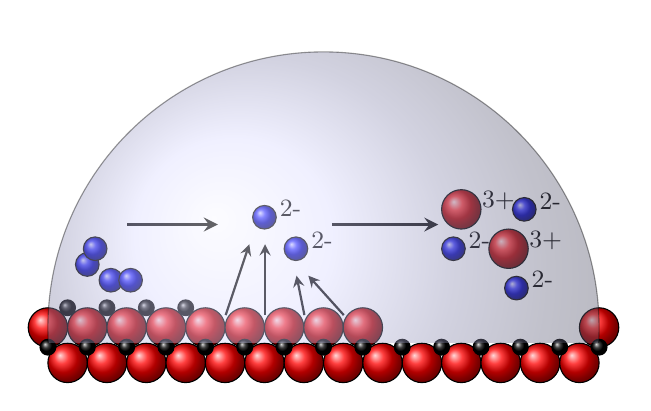
\begin{tikzpicture}[
        >=stealth,
        iron/.style={shade, ball color=red},
        electron/.style={shade, ball color=black},
        oxygen/.style={shade, ball color=blue},
        droplet/.style={ball color=blue!20, opacity=0.4},
    ]

    %Draw the iron atoms
    \foreach \x in {1,1.5,2,2.5,3,3.5,4,4.5,5,8}
            \draw [iron] (\x,1,-0.5) circle (0.25cm);
    \foreach \x in {1.25,1.75,2.25,2.75,3.25,3.75,4.25,4.75,5.25,5.75,6.25,6.75,7.25,7.75}
            \draw [iron] (\x,0.55,-0.5) circle (0.25cm);

    %Draw the iron electrons; this isn't totally realistic for illustrating Fe+3 ions
    \foreach \x in {1.25,1.75,2.25,2.75}
            \draw [electron] (\x,1.25,-0.5) circle (0.1cm);
    \foreach \x in {1,1.5,2,2.5,3,3.5,4,4.5,5,5.5,6,6.5,7,7.5,8}
            \draw [electron] (\x,0.75,-0.5) circle (0.1cm);

    %Draw the O2 molecules
    \draw [oxygen] (1.5,1.8,-0.5) circle (0.15cm);
    \draw [oxygen] (1.6,2.0,-0.5) circle (0.15cm);

    \draw [oxygen] (1.8,1.6,-0.5) circle (0.15cm);
    \draw [oxygen] (2.05,1.6,-0.5) circle (0.15cm);

    %Draw the arrows showing the electrons going to the O2 molecules
    \draw (3.45,1.35) -- (3.75,2.25) [->,thick];
    \draw (3.95,1.35) -- (3.95,2.25) [->,thick];
    \draw (4.45,1.35) -- (4.35,1.85) [->,thick];
    \draw (4.95,1.35) -- (4.5,1.85) [->,thick];

    %Draw O-2 ions with (-) labels
    \shadedraw [oxygen] (3.75,2.4,-0.5) circle (0.15cm) node [above=3pt,right=2pt] {\small{2-}};
    \shadedraw [oxygen] (4.15,2.0,-0.5) circle (0.15cm) node [above=3pt,right=2pt] {\small{2-}};

    %Draw the dissolved Fe+3 ions and O-2 ions
    \shadedraw [iron] (6.25,2.5,-0.5) circle (0.25cm) node [above=3pt,right=4pt] {\small{3+}};
    \shadedraw [iron] (6.85,2.0,-0.5) circle (0.25cm) node [above=3pt,right=4pt] {\small{3+}};

    \shadedraw [oxygen] (6.95,1.5,-0.5) circle (0.15cm) node [above=3pt,right=2pt] {\small{2-}};
    \shadedraw [oxygen] (6.15,2.0,-0.5) circle (0.15cm) node [above=3pt,right=2pt] {\small{2-}};
    \shadedraw [oxygen] (7.05,2.5,-0.5) circle (0.15cm) node [above=3pt,right=2pt] {\small{2-}};

    %Draw the time arrows
    \draw (2.2,2.5) -- (3.35,2.5) [->,very thick];
    \draw (4.8,2.5) -- (6.15,2.5) [->,very thick];

    %Draw the water droplet
    \begin{scope}
            \clip (1,1) rectangle (8.5,5);
            \draw[droplet] (4.5,1,-0.5) circle (3.5cm);
    \end{scope}
    \end{tikzpicture}
\caption{Slicica}
\end{figure}


% ukljuci >> dodatak/dodataka_b.tex <<
%\input{dodatak/dodatak_b}
% ukljuci >> dodatak/dodataka_c.tex <<
%% \appendix


% \addcontentsline{toc}{chapter}{Abstract}
\chapter{Prezentacija rezultata}$~$

Rezultate dobijene u simulacijama ili mjerenjima moguće je prikazati koristeći \textit{tikzpicture} makro. Ukoliko se radi o simulaciji, rezultate je potrebno spremiti u zaseban tekstualni file (\textit{testsim.txt}) pri čemu su vrijednosti za odrinatu i apscisu zapisani u kolone. Primjer formiranja jednog takvog file-a u Matlab/Octave je dat u nastavku.
 
\setlistingmatlab
\begin{lstlisting}
clear all
close all
clc

Ac=10;
f_c=500;
t=0:0.0001:0.4;
x=0.3*sin(10*pi*t)+0.2*sin(45*pi*t)+0.4*sin(20*pi*t);

mu=0.5;
x_c=Ac*(1+mu*x).*cos(2*pi*f_c*t);

fid=fopen('test.txt','w');
fprintf(fid,'x \t\t\t  y1  \t\t\t  y3  \t\t\t  y2  \n');
for n=1:3:2000
    fprintf(fid,'%f \t\t %f  \t\t %f  \t\t %f \n',t(n)
    ,Ac*(1+mu*x(n)),-Ac*(1+mu*x(n)),x_c(n));
end
fclose(fid);
 
\end{lstlisting}

\setlength{\parindent}{0pt}
Rezultati simulacije spremljeni su u file \textit{testsim.txt} čiji je sadržaj

\small{
\texttt{
\setlength{\parindent}{0pt}
x  \hfill		 y1 \hfill			  y3 \hfill			  y2  \\ 
0.000000\hfill 	 10.000000\hfill  -10.000000\hfill 10.000000\\ 
0.000300\hfill 	 10.094233\hfill  -10.094233\hfill $~$5.933241 \\\ 
0.000600\hfill 	 10.188374\hfill  -10.188374\hfill -3.148381 \\ 
0.000900\hfill 	 10.282334\hfill  -10.282334\hfill -9.779081 \\ 
0.001200\hfill 	 10.376022\hfill  -10.376022\hfill -8.394378 \\ 
0.001500\hfill 	 10.469348\hfill  -10.469348\hfill -0.000000 \\ 
0.001800\hfill 	 10.562222\hfill  -10.562222\hfill  $~$8.545017 \\ 
0.002100\hfill 	 10.654556\hfill  -10.654556\hfill  10.133085 \\ 
0.002400\hfill 	 10.746261\hfill  -10.746261\hfill  $~$3.320777 \\ 
0.002700\hfill 	 10.837251\hfill  -10.837251\hfill  -6.369976 \\ 
0.003000\hfill 	 10.927439\hfill  -10.927439\hfill  -10.927439 \\ 
0.003300\hfill 	 11.016742\hfill  -11.016742\hfill  -6.475479 \\ 
0.003600\hfill 	 11.105076\hfill  -11.105076\hfill  $~$3.431657 \\ 
0.003900\hfill 	 11.192359\hfill  -11.192359\hfill  10.644566 \\ 
}}


Primjer prezentacije rezultata iz file \textit{testsim.txt} koristeći \textit{tikzpicture} makro dat je u izvornom file-u \textit{dodatak\_c.tex}.

\begin{figure}[H] 
	\centering
	\begin{tikzpicture}[scale=0.8]
			\begin{axis}[width=19cm,height=8cm,xmin=0,xmax=0.2,grid=major,xlabel=$t(s)$,ylabel= $x_{mod}(t)$]
				\addplot[color=red,line width=1pt] table[x=x,y=y1] {slike/testsim.txt};
				\addplot[color=white,line width=0.5pt,draw=blue!80!white] table[x=x,y=y2] {slike/testsim.txt};
				\addplot[smooth,color=red,line width=1pt] table[x=x,y=y3] {slike/testsim.txt};
			\end{axis}
	\end{tikzpicture}
	
	\caption{} 
\end{figure}


%\input{instalacija} 
%


\end{document}

